\documentclass[tikz,border=8pt]{standalone}
\usepackage{tikz}
\usetikzlibrary{positioning,calc}

\begin{document}
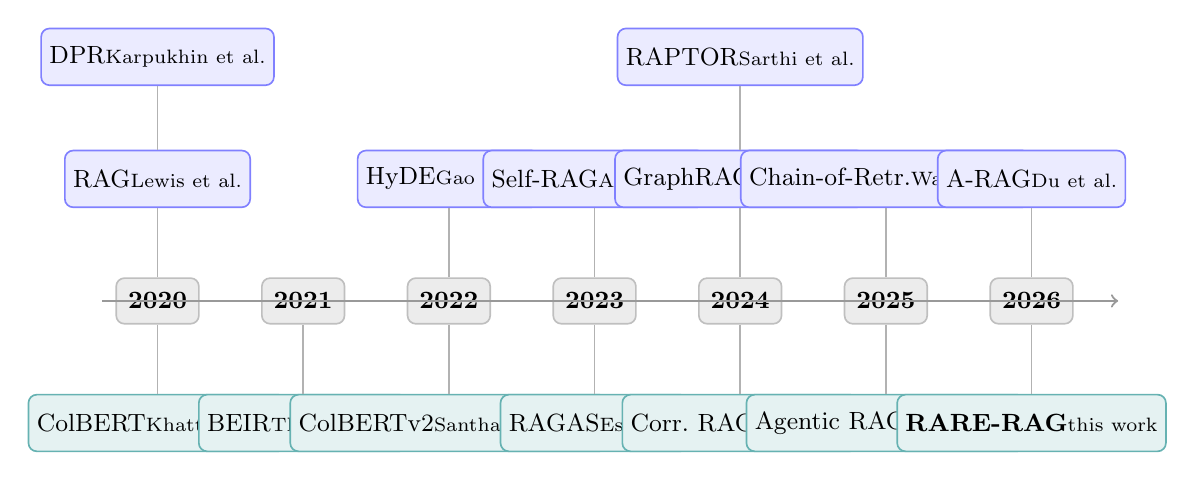
\begin{tikzpicture}[
  bluebox/.style={
    draw=blue!50, fill=blue!8, rounded corners=3pt,
    text centered, minimum width=1.55cm, minimum height=0.72cm,
    inner sep=3pt, font=\small, line width=0.6pt
  },
  tealbox/.style={
    draw=teal!60, fill=teal!10, rounded corners=3pt,
    text centered, minimum width=1.55cm, minimum height=0.72cm,
    inner sep=3pt, font=\small, line width=0.6pt
  },
  yearbox/.style={
    draw=gray!50, fill=gray!15, rounded corners=3pt,
    text centered, minimum width=1.05cm, minimum height=0.58cm,
    font=\small\bfseries, line width=0.6pt
  },
  conn/.style={gray!60, line width=0.6pt},
]

%% Year boxes on the axis (y=0)
\node[yearbox] (y0) at (0,   0) {\textbf{2020}};
\node[yearbox] (y1) at (1.85,0) {\textbf{2021}};
\node[yearbox] (y2) at (3.70,0) {\textbf{2022}};
\node[yearbox] (y3) at (5.55,0) {\textbf{2023}};
\node[yearbox] (y4) at (7.40,0) {\textbf{2024}};
\node[yearbox] (y5) at (9.25,0) {\textbf{2025}};
\node[yearbox] (y6) at (11.1,0) {\textbf{2026}};

%% Timeline axis
\draw[->, thick, gray!80] (-0.7,0) -- (12.2,0);

%% Upper row 1 (blue, y=1.55)
\node[bluebox] (rag)      at (0,   1.55) {RAG\\{\scriptsize Lewis et al.}};
\node[bluebox] (hyde)     at (3.70,1.55) {HyDE\\{\scriptsize Gao et al.}};
\node[bluebox] (selfrag)  at (5.55,1.55) {Self-RAG\\{\scriptsize Asai et al.}};
\node[bluebox] (graphrag) at (7.40,1.55) {GraphRAG\\{\scriptsize Edge et al.}};
\node[bluebox] (chain)    at (9.25,1.55) {Chain-of-Retr.\\{\scriptsize Wang et al.}};
\node[bluebox] (arag)     at (11.1,1.55) {A-RAG\\{\scriptsize Du et al.}};

%% Upper row 2 (blue, y=3.10) — stacked above DPR→RAG and RAPTOR→GraphRAG
\node[bluebox] (dpr)    at (0,   3.10) {DPR\\{\scriptsize Karpukhin et al.}};
\node[bluebox] (raptor) at (7.40,3.10) {RAPTOR\\{\scriptsize Sarthi et al.}};

%% Lower row (teal, y=-1.55)
\node[tealbox] (colbert)   at (0,   -1.55) {ColBERT\\{\scriptsize Khattab \& Z.}};
\node[tealbox] (beir)      at (1.85,-1.55) {BEIR\\{\scriptsize Thakur et al.}};
\node[tealbox] (colbertv2) at (3.70,-1.55) {ColBERTv2\\{\scriptsize Santhanam et al.}};
\node[tealbox] (ragas)     at (5.55,-1.55) {RAGAS\\{\scriptsize Es et al.}};
\node[tealbox] (corrrag)   at (7.40,-1.55) {Corr.\ RAG\\{\scriptsize Yan et al.}};
\node[tealbox] (agentic)   at (9.25,-1.55) {Agentic RAG\\{\scriptsize Singh et al.}};
\node[tealbox] (rarerag)   at (11.1,-1.55) {\textbf{RARE-RAG}\\{\scriptsize this work}};

%% Connections: chained vertically (axis→row1→row2 without crossing boxes)
\draw[conn] (y0.north)       -- (rag.south);
\draw[conn] (rag.north)      -- (dpr.south);   %% chain: axis→RAG→DPR

\draw[conn] (y4.north)       -- (graphrag.south);
\draw[conn] (graphrag.north) -- (raptor.south); %% chain: axis→GraphRAG→RAPTOR

%% Single upper connections
\draw[conn] (y2.north) -- (hyde.south);
\draw[conn] (y3.north) -- (selfrag.south);
\draw[conn] (y5.north) -- (chain.south);
\draw[conn] (y6.north) -- (arag.south);

%% Lower connections
\draw[conn] (y0.south) -- (colbert.north);
\draw[conn] (y1.south) -- (beir.north);
\draw[conn] (y2.south) -- (colbertv2.north);
\draw[conn] (y3.south) -- (ragas.north);
\draw[conn] (y4.south) -- (corrrag.north);
\draw[conn] (y5.south) -- (agentic.north);
\draw[conn] (y6.south) -- (rarerag.north);

\end{tikzpicture}
\end{document}
